\documentclass[12pt,a4paper,notitlepage]{article}
% \documentclass[conf]{new-aiaa}
\usepackage[framed,numbered,autolinebreaks]{mcode}
\usepackage[margin=1in]{geometry}
\usepackage{amsmath}
\usepackage{amsfonts}
\usepackage{amssymb}
\usepackage{graphicx}
\usepackage{color}
\usepackage{float}
\usepackage[toc,page]{appendix}
\usepackage{parskip}
\usepackage{sectsty}
\usepackage{gensymb}
\usepackage{titlesec}
\usepackage{listings}
% \lstset{language=Matlab,%
%     %basicstyle=\color{red},
%     breaklines=true,%
%     morekeywords={matlab2tikz},
%     keywordstyle=\color{blue},%
%     morekeywords=[2]{1}, keywordstyle=[2]{\color{black}},
%     identifierstyle=\color{black},%
%     stringstyle=\color{mylilas},
%     commentstyle=\color{mygreen},%
%     showstringspaces=false,%without this there will be a symbol in the places where there is a space
%     numbers=left,%
%     numberstyle={\tiny \color{black}},% size of the numbers
%     numbersep=9pt, % this defines how far the numbers are from the text
%     emph=[1]{for,end,break},emphstyle=[1]\color{red}, %some words to emphasise
%     %emph=[2]{word1,word2}, emphstyle=[2]{style},    
% }
\usepackage{titling}
\setlength{\droptitle}{-1cm}
\usepackage{enumitem}
\usepackage{multirow}
\usepackage{longtable}

\usepackage[
backend=biber,
style=numeric,
sorting=none
]{biblatex}
 
\addbibresource{draft.bib}


\setlist[enumerate]{topsep=0pt,itemsep=-3.5ex,partopsep=1ex,parsep=1ex}
\renewcommand{\rmdefault}{ptm}
\sectionfont{\fontsize{12}{0}\selectfont}
\subsectionfont{\fontsize{12}{0}\selectfont}
\usepackage[font={normal,bf}]{caption}

% Header and Footer
\setlength{\headheight}{15pt} 
\usepackage{fancyhdr}
\fancypagestyle{plain}{
 \fancyhf{}
 \fancyhead[L]{AA 290: AA 279D Project}
 \fancyhead[R]{Stanford University}
 \fancyfoot[C]{\thepage}
}

% Table of contents
\setcounter{tocdepth}{5}

\begin{document}
\title{\Huge \textbf{Project Title}}
\author{\Large Ethan LeBoeuf}
\date{\Large 23 September 2019}

\begin{minipage}[h]{\textwidth}
	\vspace{4 cm}
	\advance\leftskip-1in
    \maketitle
\end{minipage}

\begin{figure}[H]
\centering
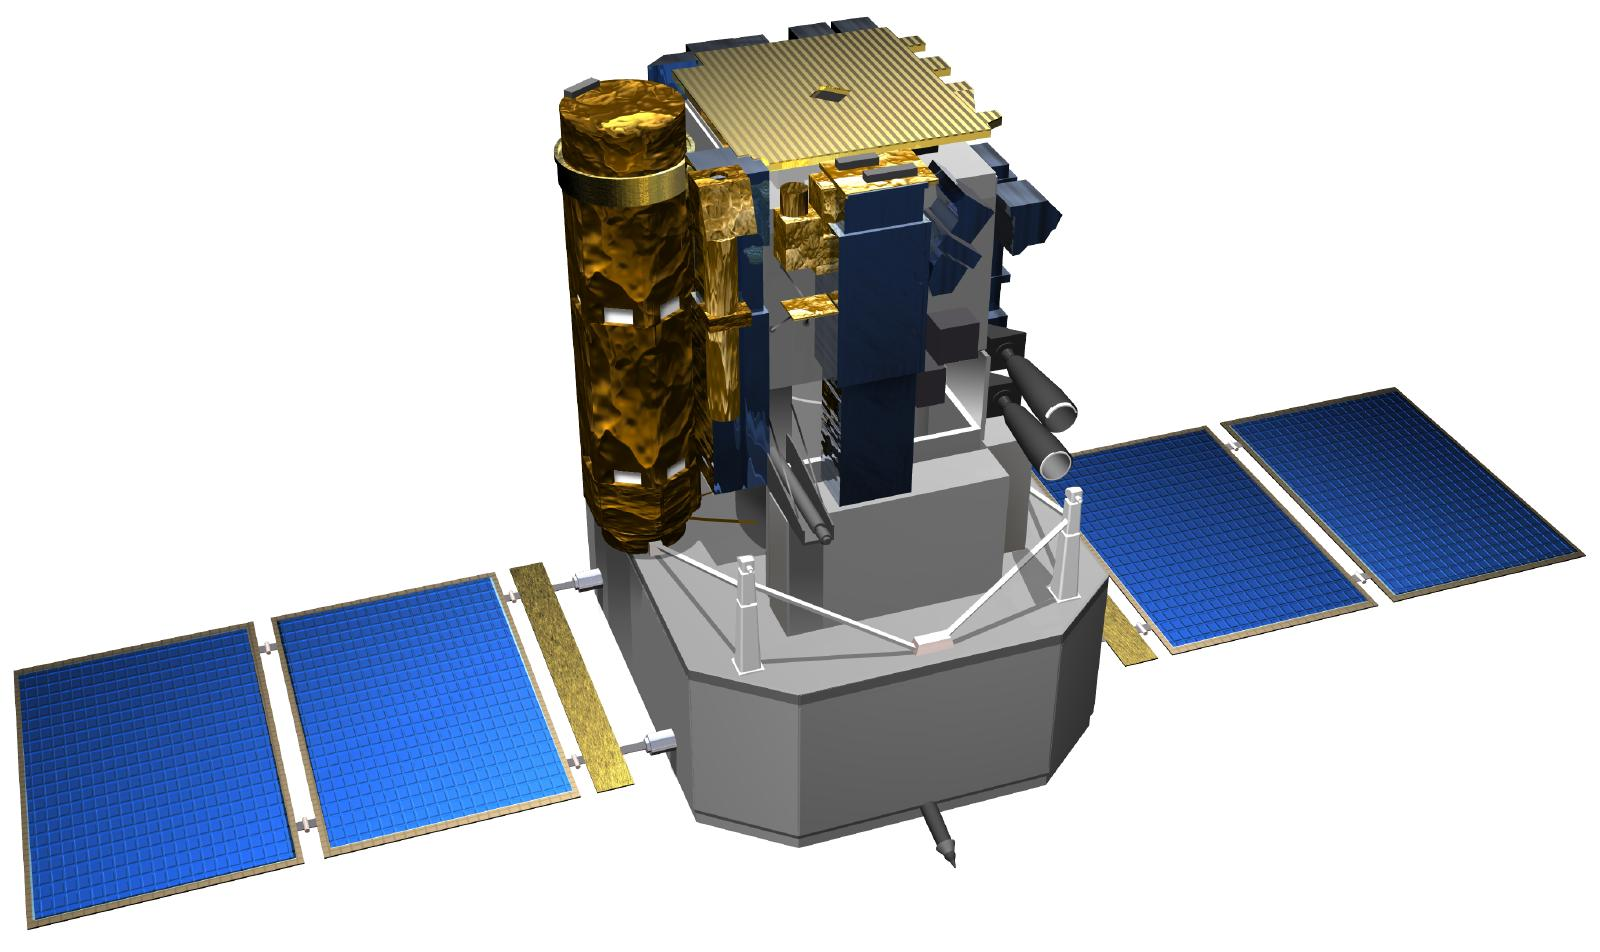
\includegraphics[scale=0.28]{Images/SOHO.jpg}
\end{figure}

\pagebreak

\section*{\Large REVISION HISTORY}

\begin{table}[h!]
\begin{center}
\begin{tabular} [0.9 \textwidth]{cl}
\hline \hline
\multicolumn{1}{c}{VERSION} & \multicolumn{1}{l}{REVISION NOTES} \\
\hline
PS1 & - Created document \\
    & - Added PS1 material \\
%  \hline
%  PS2 & - Added PS2 material \\
%  & - Updated title page \\
%  & - Added table of contents \\
%  & - Updated orbit around L2 point \\
%  & - Discretized cylindrical parts of geometry \\
\hline \hline
\end{tabular}
	\caption{Summary of project revisions.}
\end{center}
\end{table}
 
\newpage
\section*{\Large TABLE OF CONTENTS}
\makeatletter
\@starttoc{toc}
\makeatother
\newpage
%%%%%%%%%%%%%%%%%%%%%%%%%%%%%%%%%%%%%%%%%%%%%%%%%%%%%%%%%%%%%%%%%%%%%%%%%%%%%%%%%%%%%%%%%%%%%%%%%%%%%%%%%%%%%%%%%%%%%%%%%%%%%%%%%%%%%%%%%%%%%%%%%%%%%%%%%%%%%%%%%%%%%%%%%%%%%%%%%%%%%%%%%%%%%%%%%%%%%%%%%%%%%%%%%%%%%%%%%%%

% \section{\Large INTRODUCTION}

\section{\Large PROBLEM SET 1}
\subsection{PROBLEM 1}
Distributed systems have many uses in space. Main categories of missions using distributed systems include rendezvous and docking, formation-flying, and constellations. For this project, I initially looked into all 3 categories, but down selected to rendezvous/docking and formation flying to look into more carefully. This led me to research the Orbital Express mission, a rendezvous and docking mission done by DARPA, and the Magnetospheric Multiscale mission, a formation flying mission done by NASA. I have chosen to move forward with the Orbital Express mission as my basis as it aligns more with my interests in the field. 

The mission overview can be seen in Table \ref{table:mission_overview}.

\begin{table}[h!]
\begin{center}
\begin{tabular}{ |c|c| }
 \hline
 \textbf{Name} & Orbital Express \\ \hline
 \textbf{Agency} & DARPA \\ \hline
 \textbf{Primary Mission} & Demonstrate automated rendezvous and docking capabilities \\ \hline
 \textbf{Secondary Mission} & Demonstrate automated servicing capabilities \\ \hline
 \textbf{Number of Satellites} & 2 \\ \hline
 \textbf{Types of Satellites} & One servicing and one test \\ \hline
 \textbf{Classification of Mission} & Rendezvous and Docking \\
 \hline
\end{tabular}
\caption{Mission overview for Orbital Express}
\label{table:mission_overview}
\end{center}
\end{table}

The two satellites for the Orbital Express mission were a servicing satellite (named Astro) and a test satellite (named NextSat). Astro would perform automated docking and servicing to demonstrate these capabilities in space. Astro would dock with NextSat and then undock multiple times to show the various capabilities. Rendezvous and docking requires extremely accurate GNC capabilities as missteps can lead to catastrophic mission failure. Navigation will have to be in the centimeter accuracy for relative distances, and the controller will have to be very precise as well.  In this project I will try to demonstrate the capabilities of this mission from the beginning of the mission (kilometers away) to the final rendezvous/docking (meters away). I may also try to combine this project with aspects of my 279C project to include rotational motion to demonstrate the docking but this is a stretch goal. 

The initial orbit of Astro was near-circular orbital elements shown in Table \ref{table:orbital_elements}. The Argument of Periapsis was assumed to be 0\(\degree\) initially as it wasn't given.

\begin{table}[h!]
\begin{center}
\begin{tabular}{ |c|c| }
 \hline
 \textbf{Apogee} & 6869 km \\ \hline
 \textbf{Perigee} & 6862 km \\ \hline
 \textbf{Inclination} & 46.00\(\degree\) \\ \hline
 \textbf{Eccentricity} & 0.0005 \\ \hline
 \textbf{Argument of Perigee} & 0\(\degree\) \\ \hline
 \textbf{Launch Date} & March 9\textsuperscript{th}, 2007 \\ \hline
\end{tabular}
\caption{Orbital Elements for Orbital Express \cite{astro}}
\label{table:orbital_elements}
\end{center}
\end{table}

To separate Astro from NetSat initially, I have arbitrarily decided to put Astro at 200 km in the R-Bar direction and 100 km in the V-Bar direction. This means that Astro is above and ahead of NetSat initially.

\subsection{PROBLEM 2}
a)Define the initial conditions for the mission you identified in Problem 1. Most likely
the initial conditions are provided in literature by a set of Keplerian orbital elements
and an initial launch date and time. You are allowed to choose some consistent initial
conditions arbitrarily if not available.

b) Treat these initial conditions as osculating quantities and compute the corresponding
initial position and velocity in the inertial frame (ECI).

c) Perform a numerical integration of the equations of motion using position and velocity
as state variables and the initial conditions from b). You should perform simulations
including and excluding J2 effects. Provide plots of the paths of your distributed space
system in the ECI frame. Note that the simulation should be long enough to appreciate
secular J2 effects, i.e. an integer multiple of the orbital period.
Hint: Check equations (2.1) and (4.93) from Alfriend.

d) Verify that your integrator performs properly by comparing output with analytical
Keplerian propagation. This is a comparison between output of b) and output of c)
excluding J2 effects. Plot the error in absolute position and velocity expressed in the
RTN frame.

Hint: You should only observe numerical integration errors. Eventually reduce inte-
grator step-size to reduce numerical errors.

e) Compute and plot osculating Keplerian orbital elements, eccentricity vector, angular
momentum vector, specific mechanical energy throughout the numerical simulations
of c). Verify and show that these quantities are constant when excluding J2 effects.
What happens when you include J2 effects instead? Are the results as expected from
averaging theory?

f) Now consider the linear differential equations for the mean classical orbital elements
[(2.115) from Alfriend] including J2 effects. Verify and show the general consistency
with the osculating elements from e).

Hint: The simulation should be at least a few orbital revolutions long since the mean
elements refer to an orbit average.

g) You could encounter some inconsistencies when comparing osculating and mean orbital
elements due the initialization procedure. In fact c) needs osculating states as inputs
and provides osculating states as outputs, whereas f) needs mean states as inputs and
provides mean states as outputs. How would you solve this problem?
\newpage
\printbibliography

\newpage
\appendix
\addappheadtotoc
\Large{\bf{\appendixname}}
\section{Matlab Code}
\subsection{PSet1 Problem 5}\label{A:P1p5}

\lstinputlisting{test.m}



\end{document}